\documentclass{UoNMCHA}
\usepackage[square,numbers]{natbib}
\usepackage{array,booktabs} % For nice tables
\usepackage{amsmath,amsfonts,amssymb} % For nice maths
\usepackage{color}
\usepackage{enumerate}
\usepackage{listings}
\usepackage{subfig}
\usepackage{hyperref}
\usepackage{csquotes}
\usepackage{glossaries}			% Glossaries
\usepackage{algorithm}			% >
\usepackage{algpseudocode}		% <
\usepackage[parfill]{parskip}   % For replacing paragraph indenting with a newline instead
\DeclareOldFontCommand{\bf}{\normalfont\bfseries}{\mathbf} % Fixes \bf isssues
\usepackage{hyperref}

\input{_content/____setup.txt}

\begin{document}

	\input{_content/00_preamble/00_titlePage.txt}

	\vspace{-5mm}
	\section*{Abstract}
	\vspace{-3mm}
		\input{_content/00_preamble/01_abstract.txt}

	\vspace{-2mm}
	\section*{Acknowledgements}
	\vspace{-3mm}
		\input{_content/00_preamble/02_acknowledgements.txt}

	\newpage\tableofcontents
	
	\newpage\listoffigures\listoftables\listofalgorithms
	
	
	\newpage\section{Introduction}
		\input{_content/00_preamble/03_introduction.txt}

	\clearpage
	\newpage\section{Background}\label{sec:Background}
		\input{_content/10_background/__intro.txt}
		\subsection{Kinematics}
			\input{_content/10_background/_kinematics.txt}
		\subsection{Numerical Optimisation}
			\input{_content/10_background/_optimisation.txt}
		\subsection{Walking}
			\input{_content/10_background/_walking.txt}
	
	\clearpage
	\newpage\section{Models}\label{sec:Models}
		\input{_content/20_modelling/20_intro.txt}
		\subsection{2D Model}
			\input{_content/20_modelling/21_2D.txt}
		\subsection{3D Model}
			\input{_content/20_modelling/22_3D.txt}
	
	\clearpage	
	\newpage\section{From Trajectory to Foot Placement}\label{sec:NovelTraj}
		\input{_content/X0_traj/X0_background.txt}
		\subsection{Concept}
			\input{_content/X0_traj/X0_concept.txt}
		%%\clearpage\subsection{ZMP Reference}
			%%\input{_content/X0_traj/X0_extension.txt}
	
	\clearpage
	\newpage\section{Quasi Static Locomotion}\label{sec:Quasi Static Locomotion}
		\input{_content/30_quasiStatic/30_concept.txt}
		\subsection{2D Model Implementation}\label{sec:2D_QS}
			\input{_content/30_quasiStatic/31_2D.txt}
		\subsection{3D Model Implementation}\label{sec:3D_QS}
			\input{_content/30_quasiStatic/32_3D.txt}
			
	\clearpage
	\newpage\section{Zero Moment Point Locomotion}\label{sec:Zero Moment Point Locomotion}
		\input{_content/40_zmp/40_concept.txt}
		\subsection{3D Linear Inverted Pendulum}
			\input{_content/40_zmp/41_zmpLIPM.txt}
		\subsection{Preview Control}
			\input{_content/40_zmp/42_previewControl.txt}
		\subsection{3D Model Implementation}\label{sec:ZMP_imp}
			\input{_content/40_zmp/43_3D.txt}
	
	\clearpage
	\newpage\section{Results}\label{sec:Results}
		\input{_content/50_results/50_TCP.txt}
		\subsection{WeBots Simulation}
			\input{_content/50_results/51_Webots.txt}
		\subsection{NuGus Robot}
			\input{_content/50_results/52_NuGus.txt}
	
	\clearpage
	\newpage\section{Conclusion}\label{sec:Conclusion}
		\input{_content/X0_conclusion.txt}
	\newpage\section{Discussion}\label{sec:Discussion}
		\input{_content/X0_discussion.txt}
	\newpage\section{Recommendations}\label{sec:Recommendations}
		\input{_content/X0_recommendation.txt}
	\section{Future Work}\label{sec:FutureWork}
		\input{_content/X1_futureWork.txt}
		

	\newpage\bibliographystyle{agsm} %% https://www.mybib.com/#/projects/XRL93q/citations
		\bibliography{FinalReport}

	\appendix
		\newpage\section{Handwritten Notes}\label{app:Hand}
		%% MATLAB DRAWN QUASI MODEL
		\begin{figure}[!h]
		    \begin{center}
		        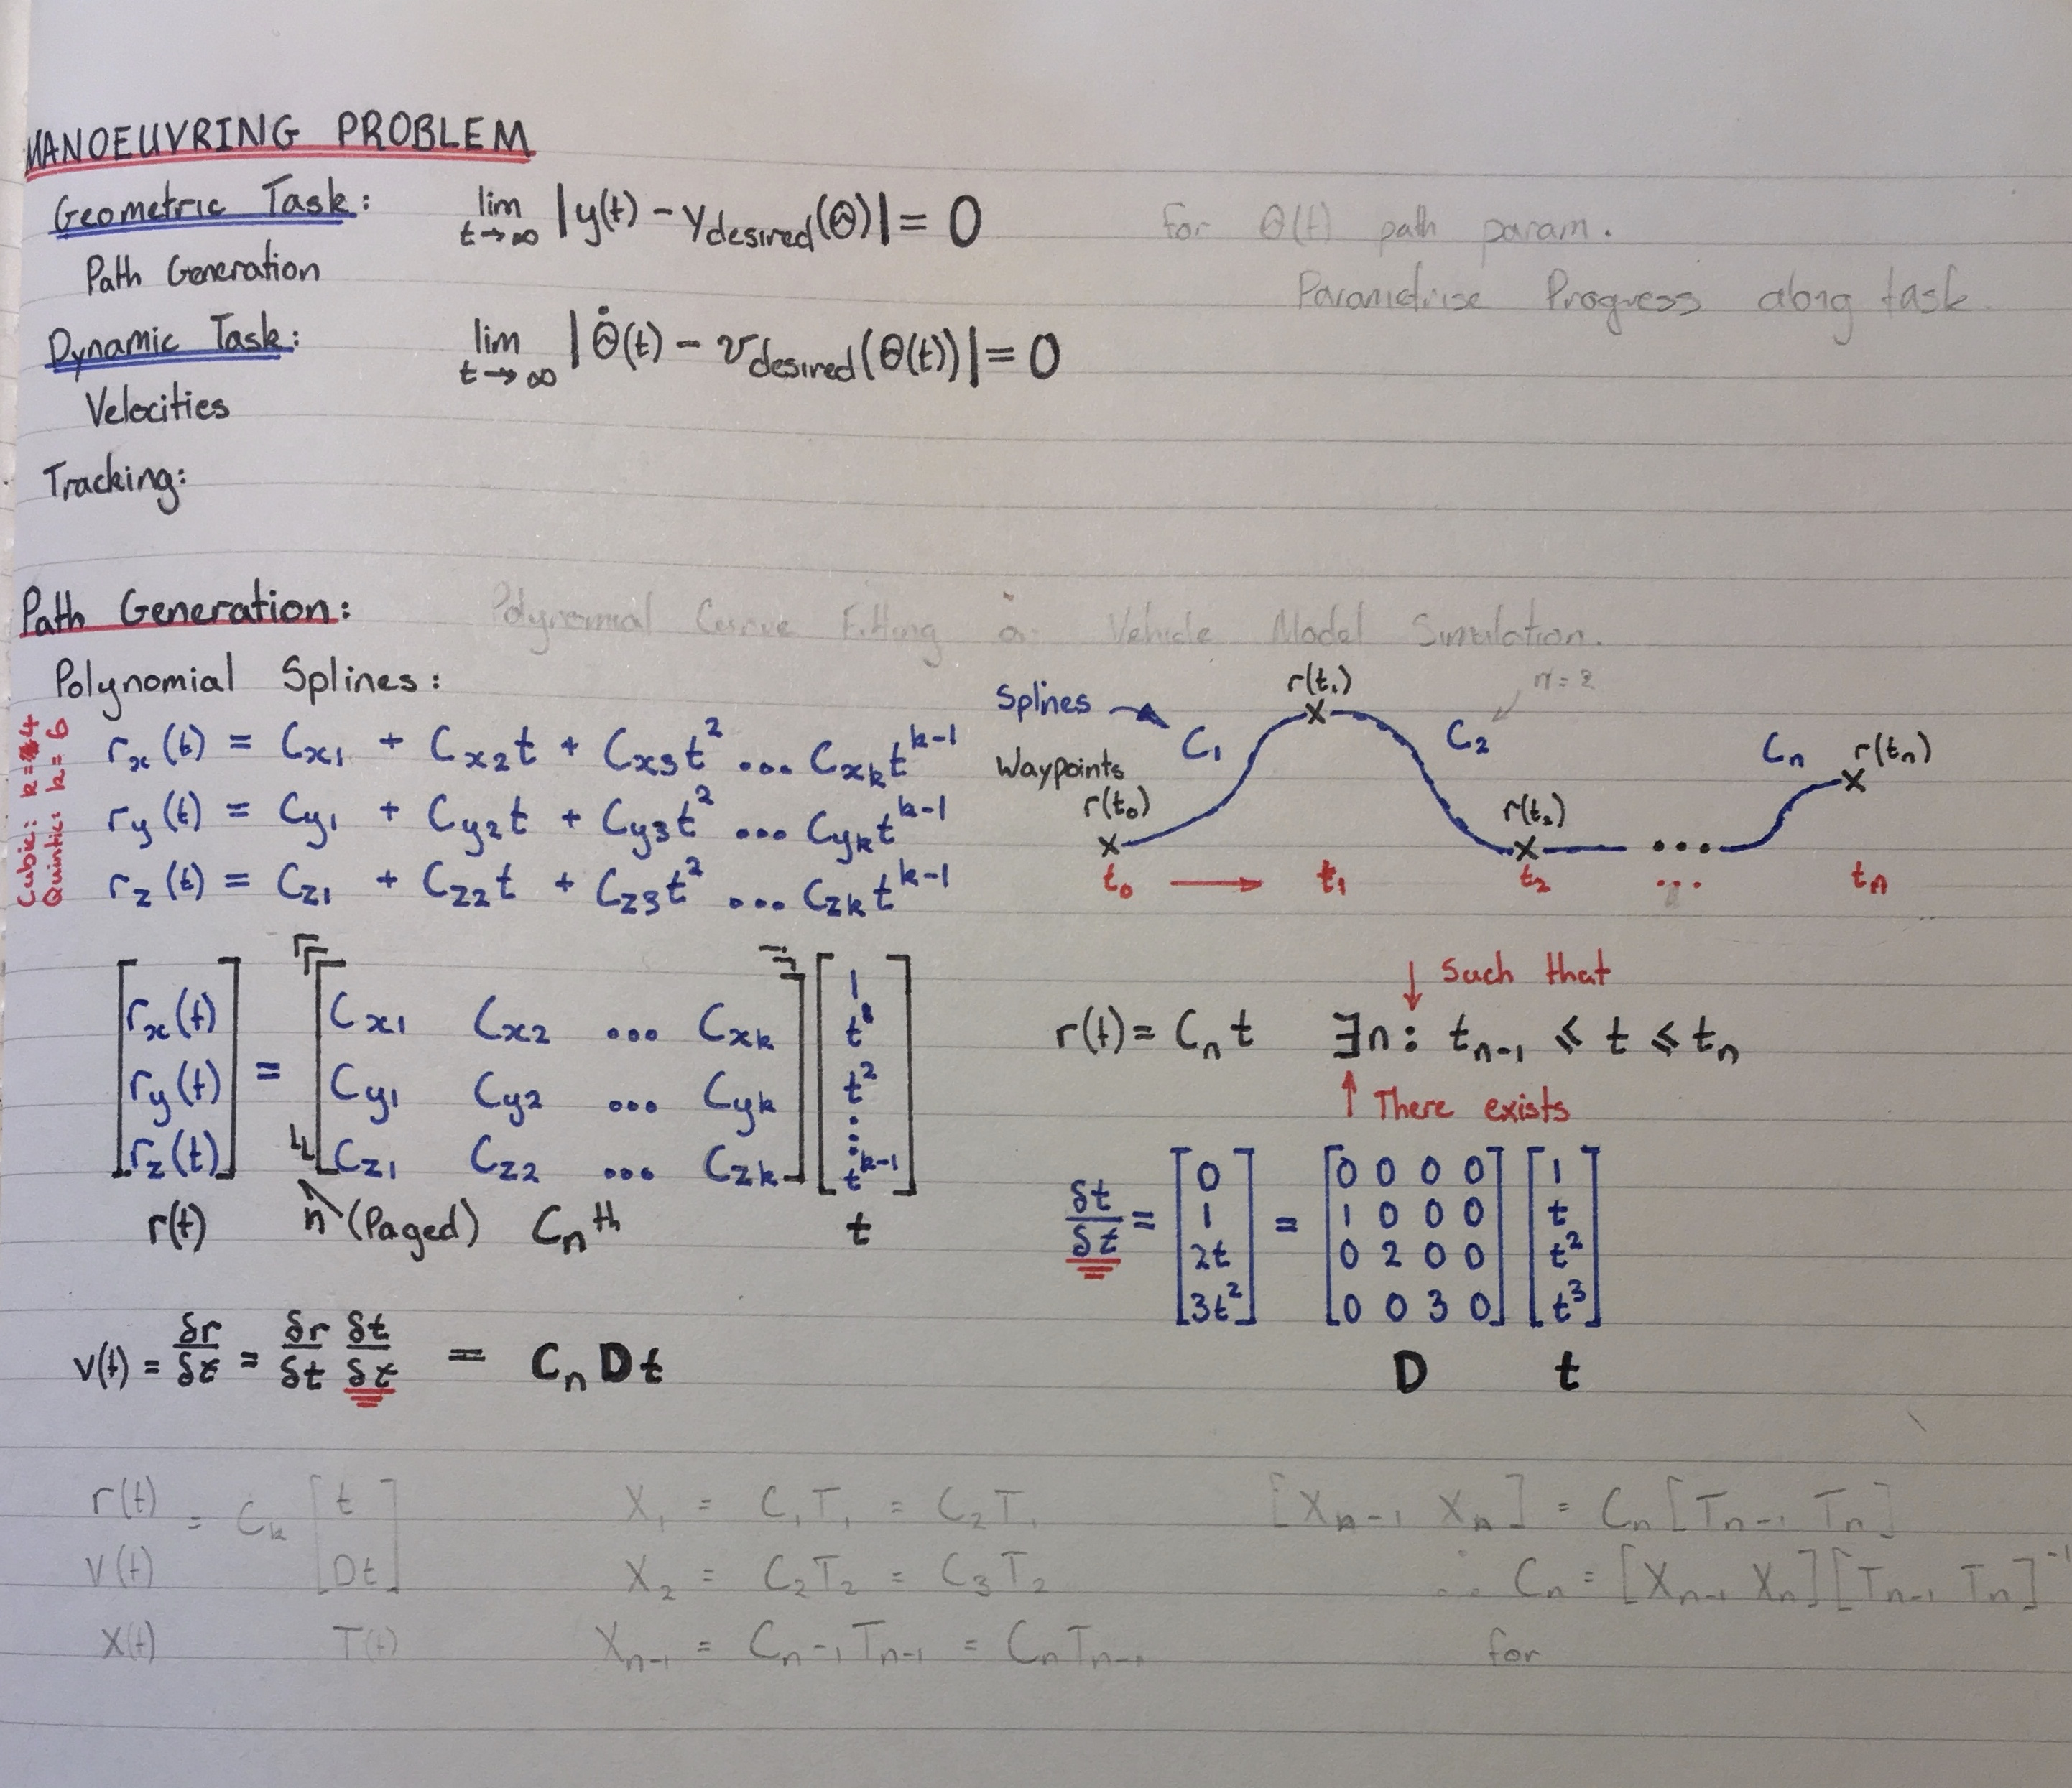
\includegraphics[width=.9\linewidth]{_figures/HAND_1_Traj.png}
		        \caption{Trajectory Generation.}
		        \label{fig:APP_TrajGen}
		    \end{center}
		\end{figure}
		\begin{figure}[!h]
		    \begin{center}
		        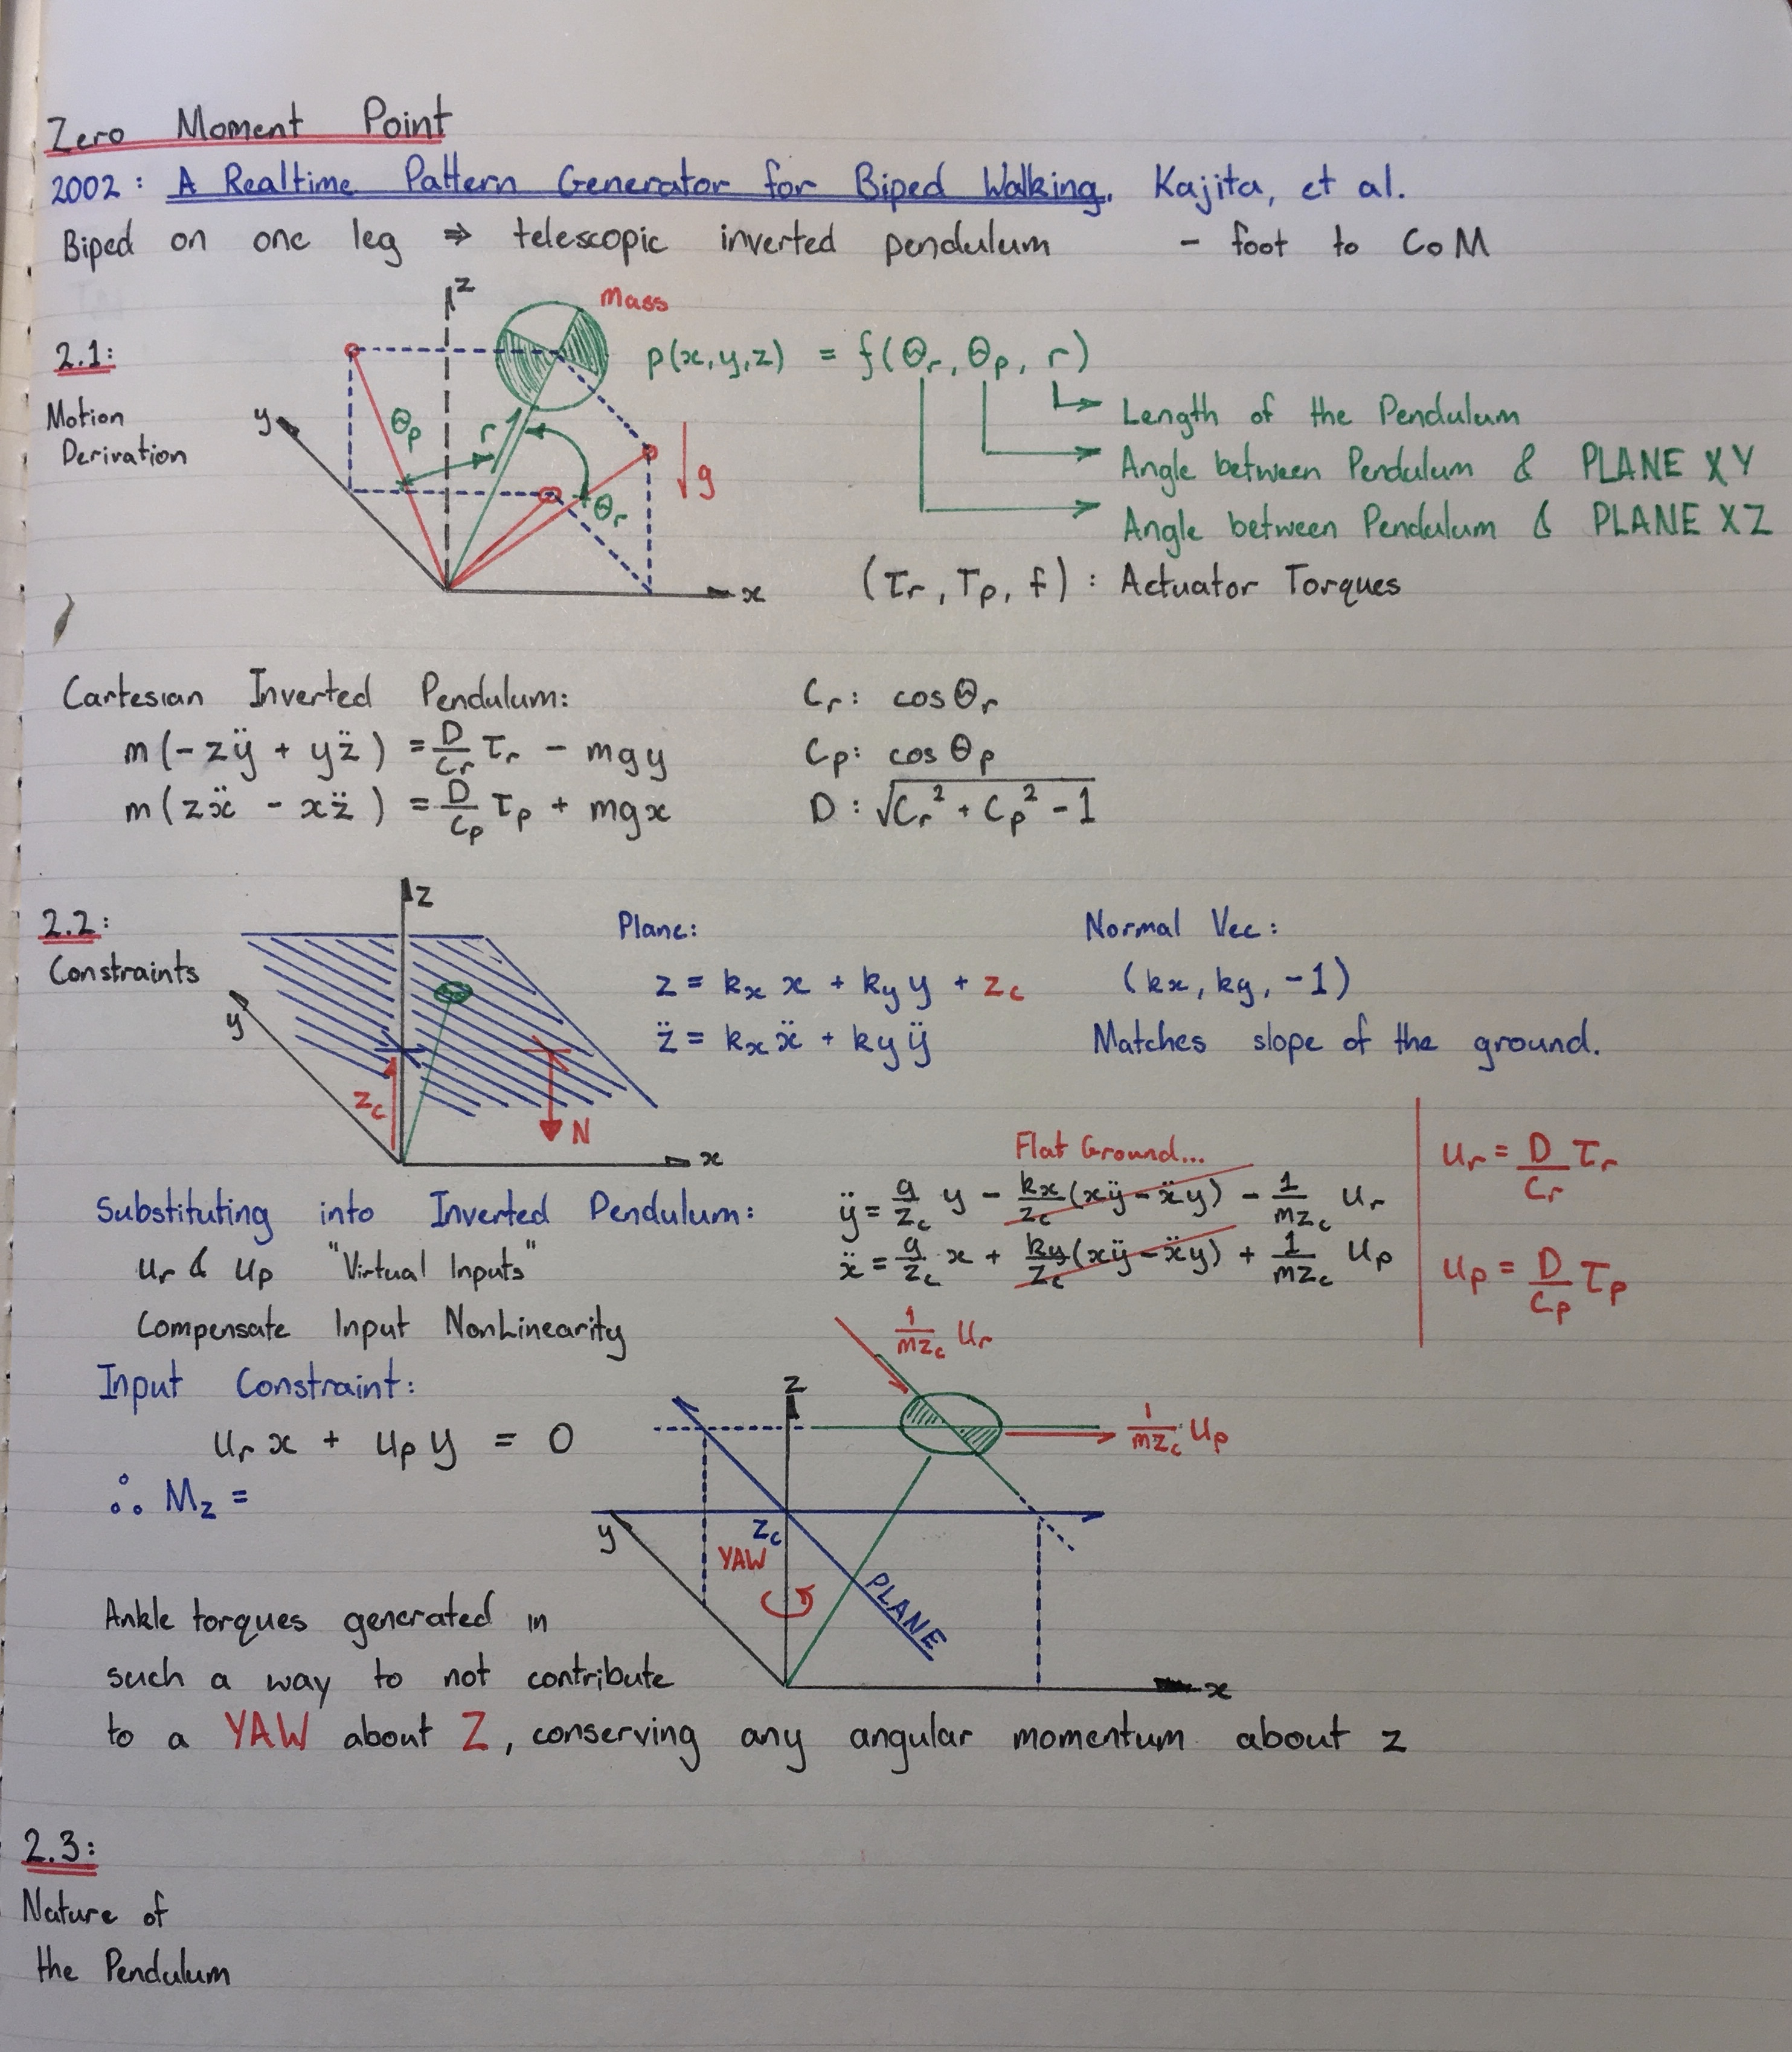
\includegraphics[width=.9\linewidth]{_figures/HAND_2_ZMP1.png}
		        \caption{ZMP1.}
		        \label{fig:APP_ZMP1}
		    \end{center}
		\end{figure}
		\begin{figure}[!h]
		    \begin{center}
		        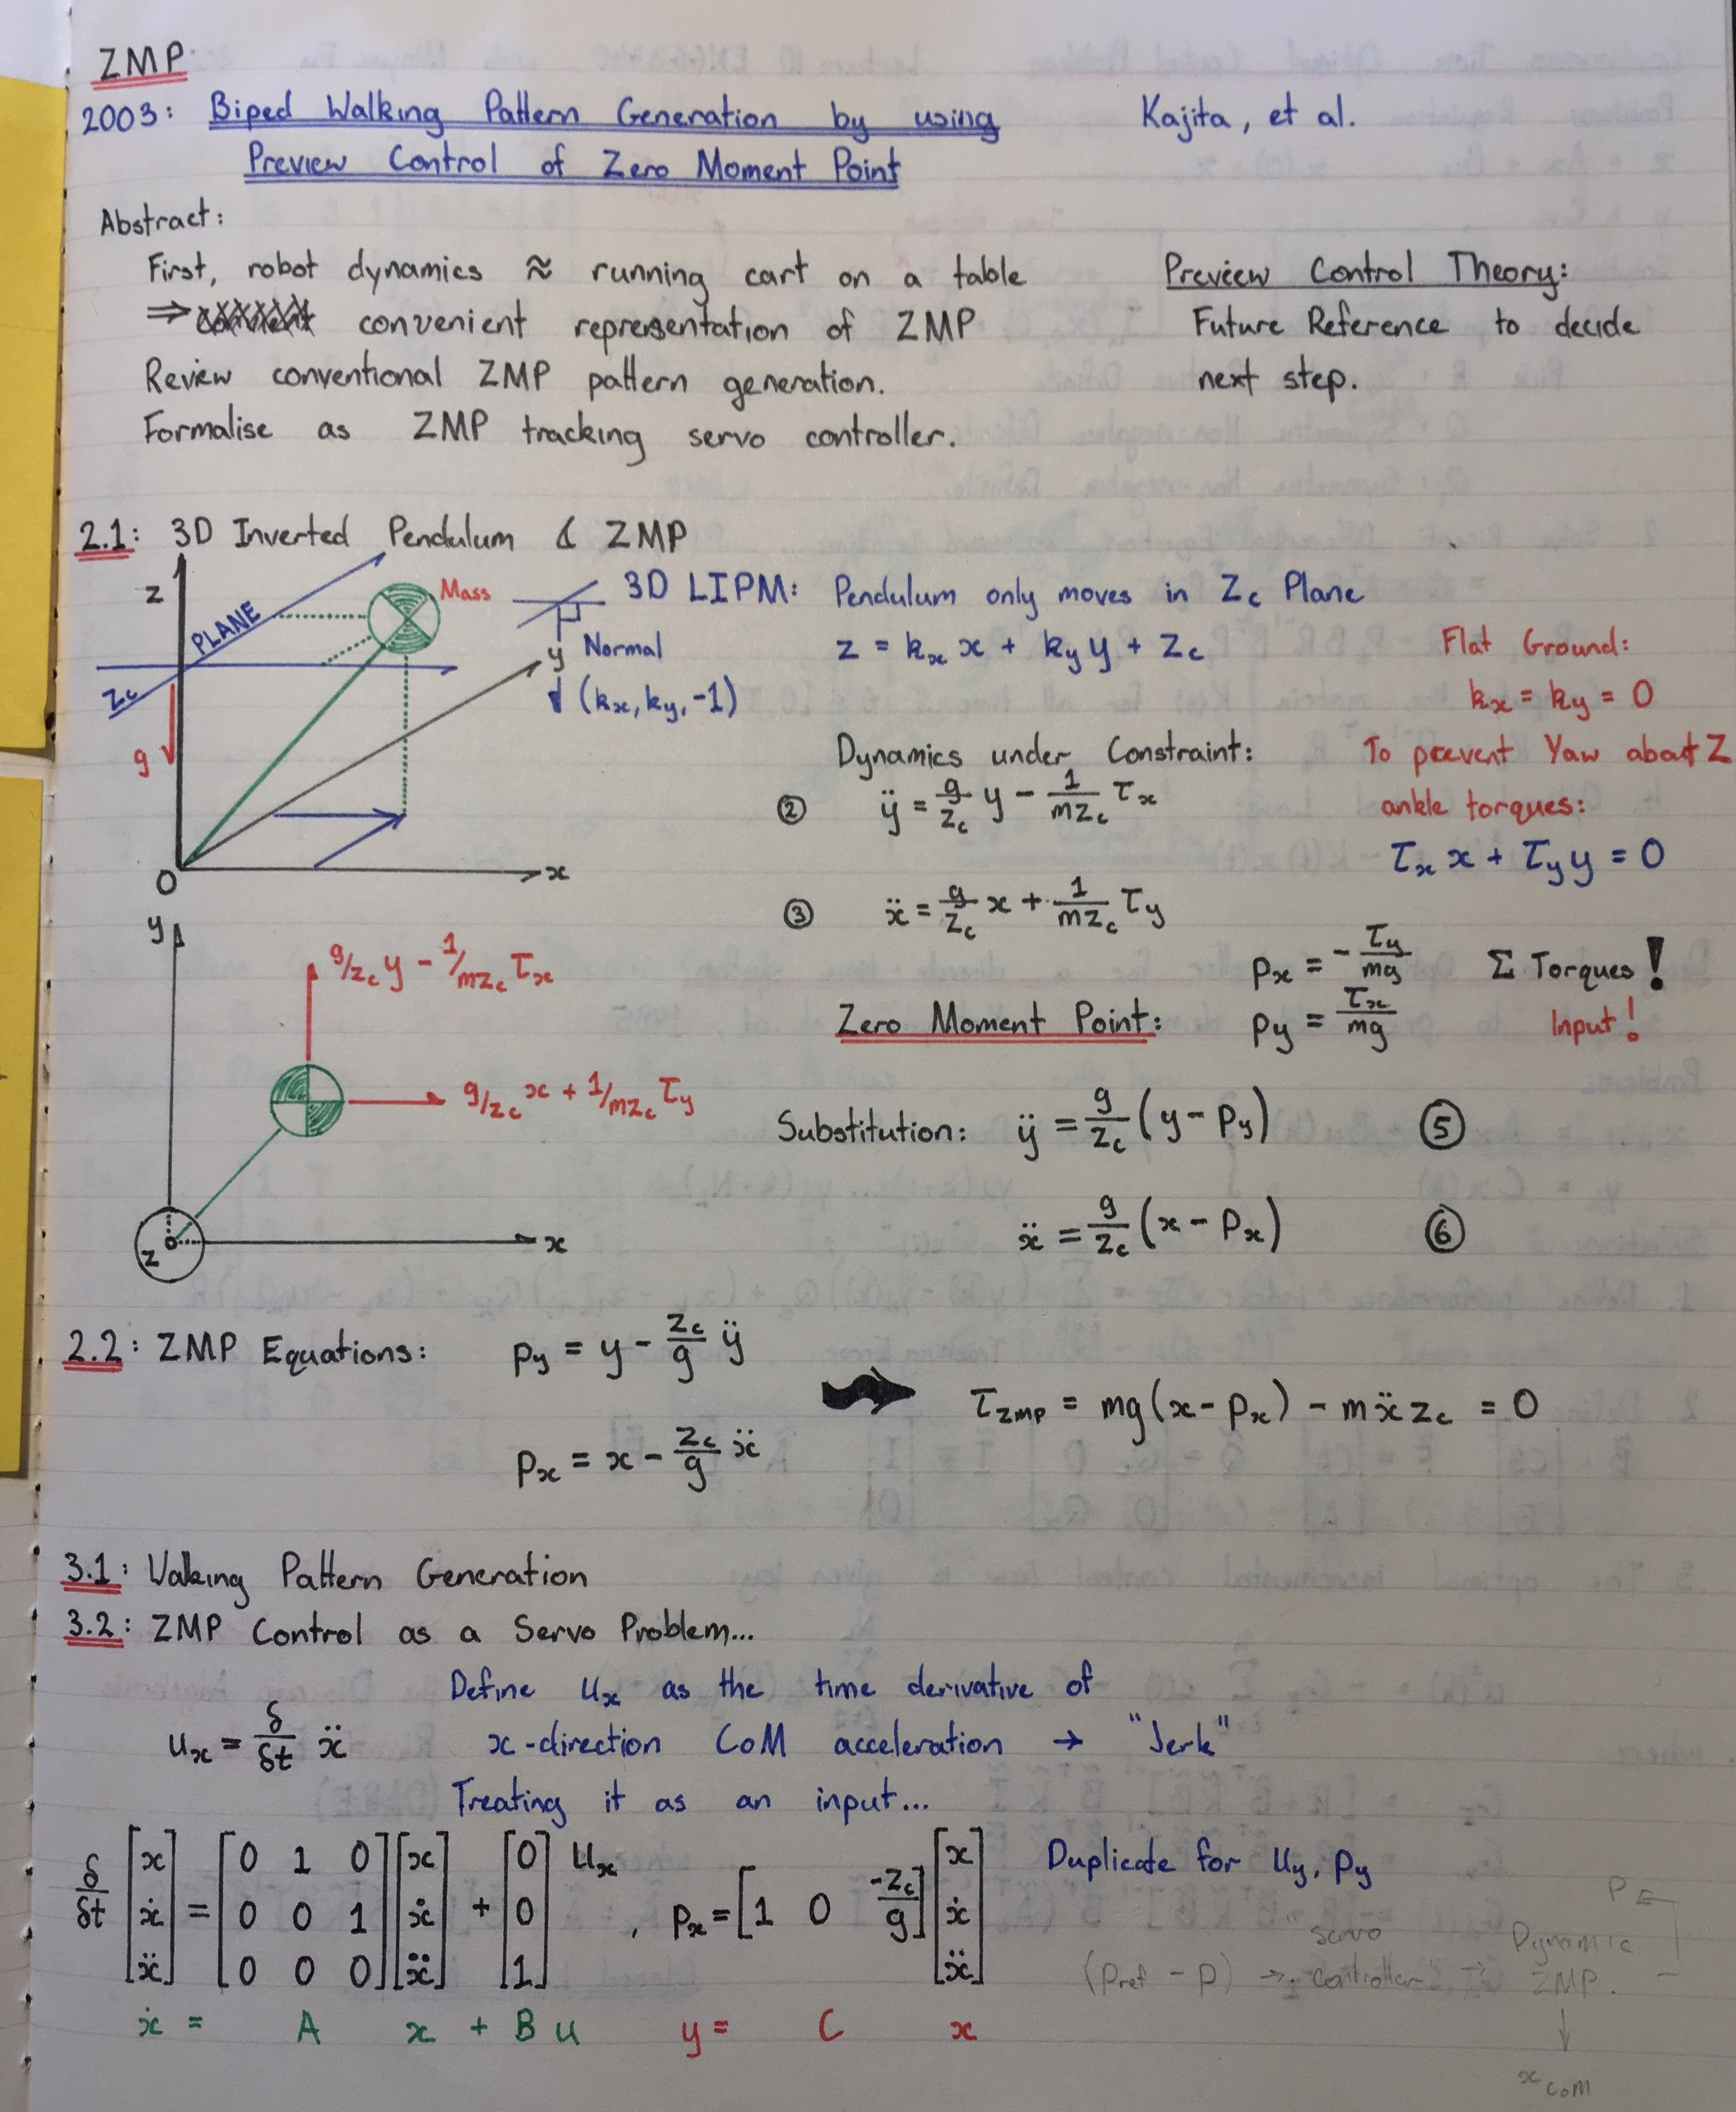
\includegraphics[width=.9\linewidth]{_figures/HAND_3_ZMP2.png}
		        \caption{ZMP2.}
		        \label{fig:APP_ZMP2}
		    \end{center}
		\end{figure}
		\begin{figure}[!h]
		    \begin{center}
		        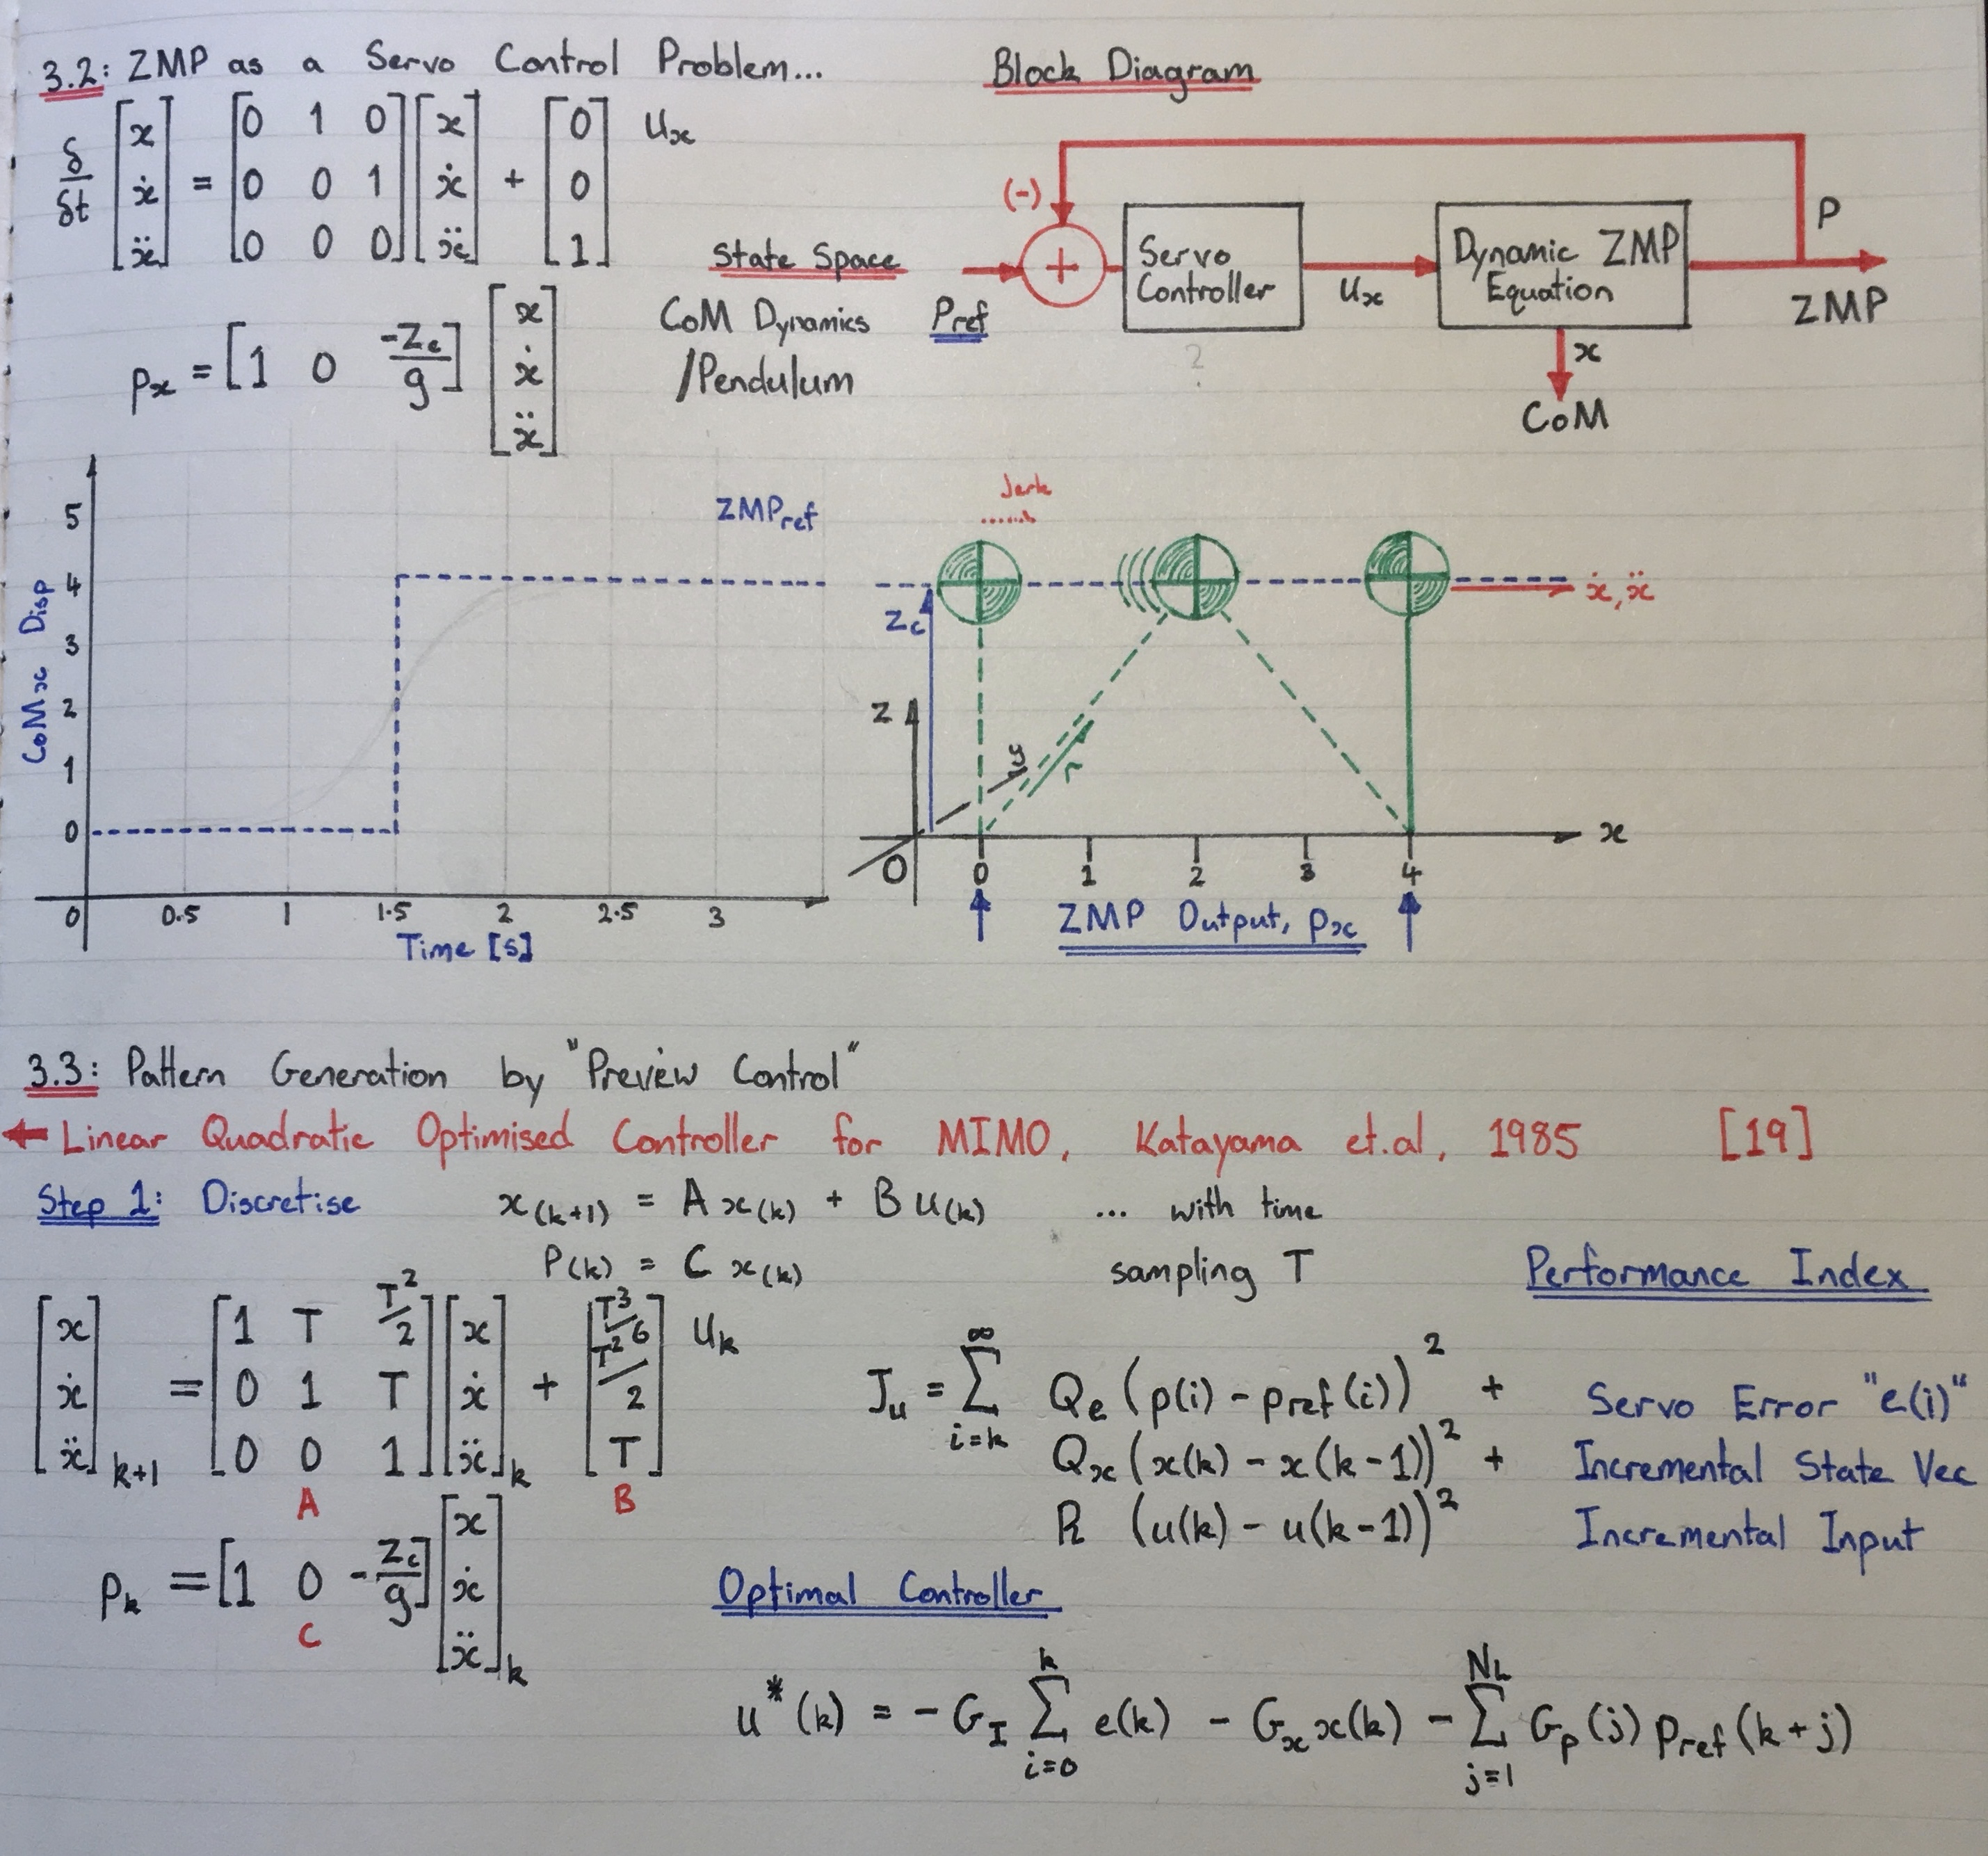
\includegraphics[width=.9\linewidth]{_figures/HAND_4_ZMP3.png}
		        \caption{ZMP3.}
		        \label{fig:APP_ZMP3}
		    \end{center}
		\end{figure}
		\begin{figure}[!h]
		    \begin{center}
		        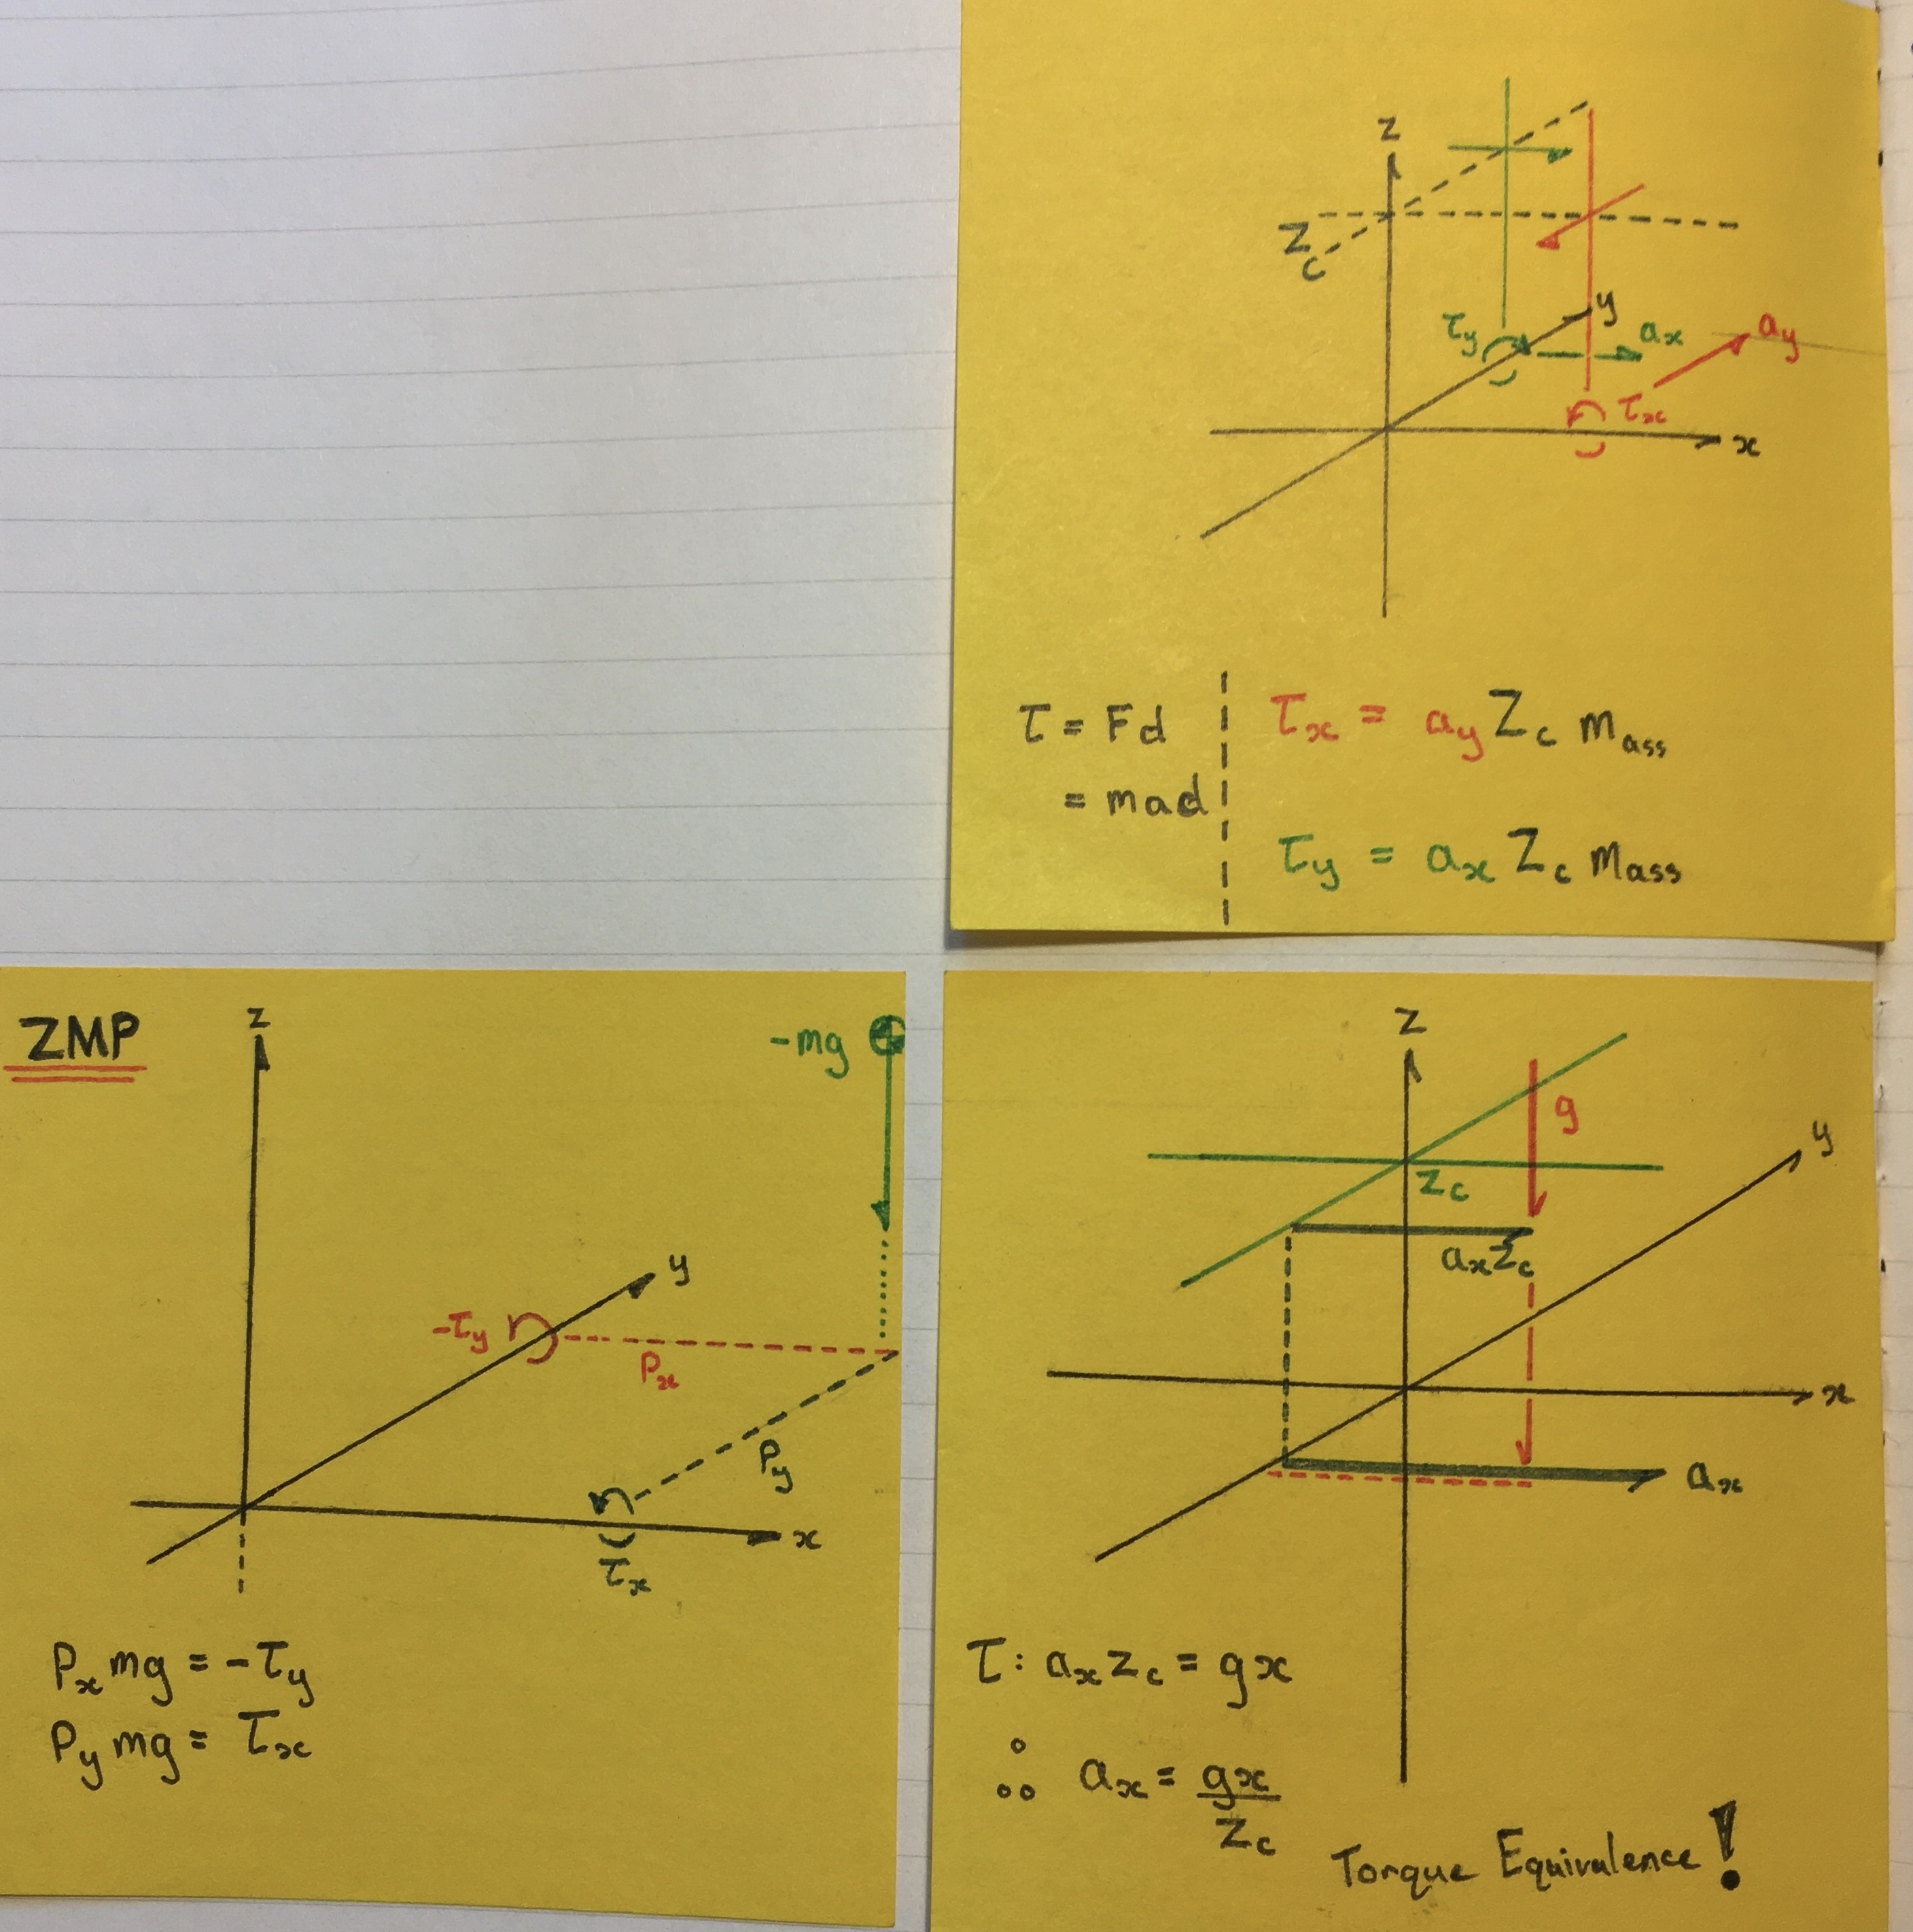
\includegraphics[width=.9\linewidth]{_figures/HAND_5_ZMP4.png}
		        \caption{ZMP4.}
		        \label{fig:APP_ZMP4}
		    \end{center}
		\end{figure}
		\begin{figure}[!h]
		    \begin{center}
		        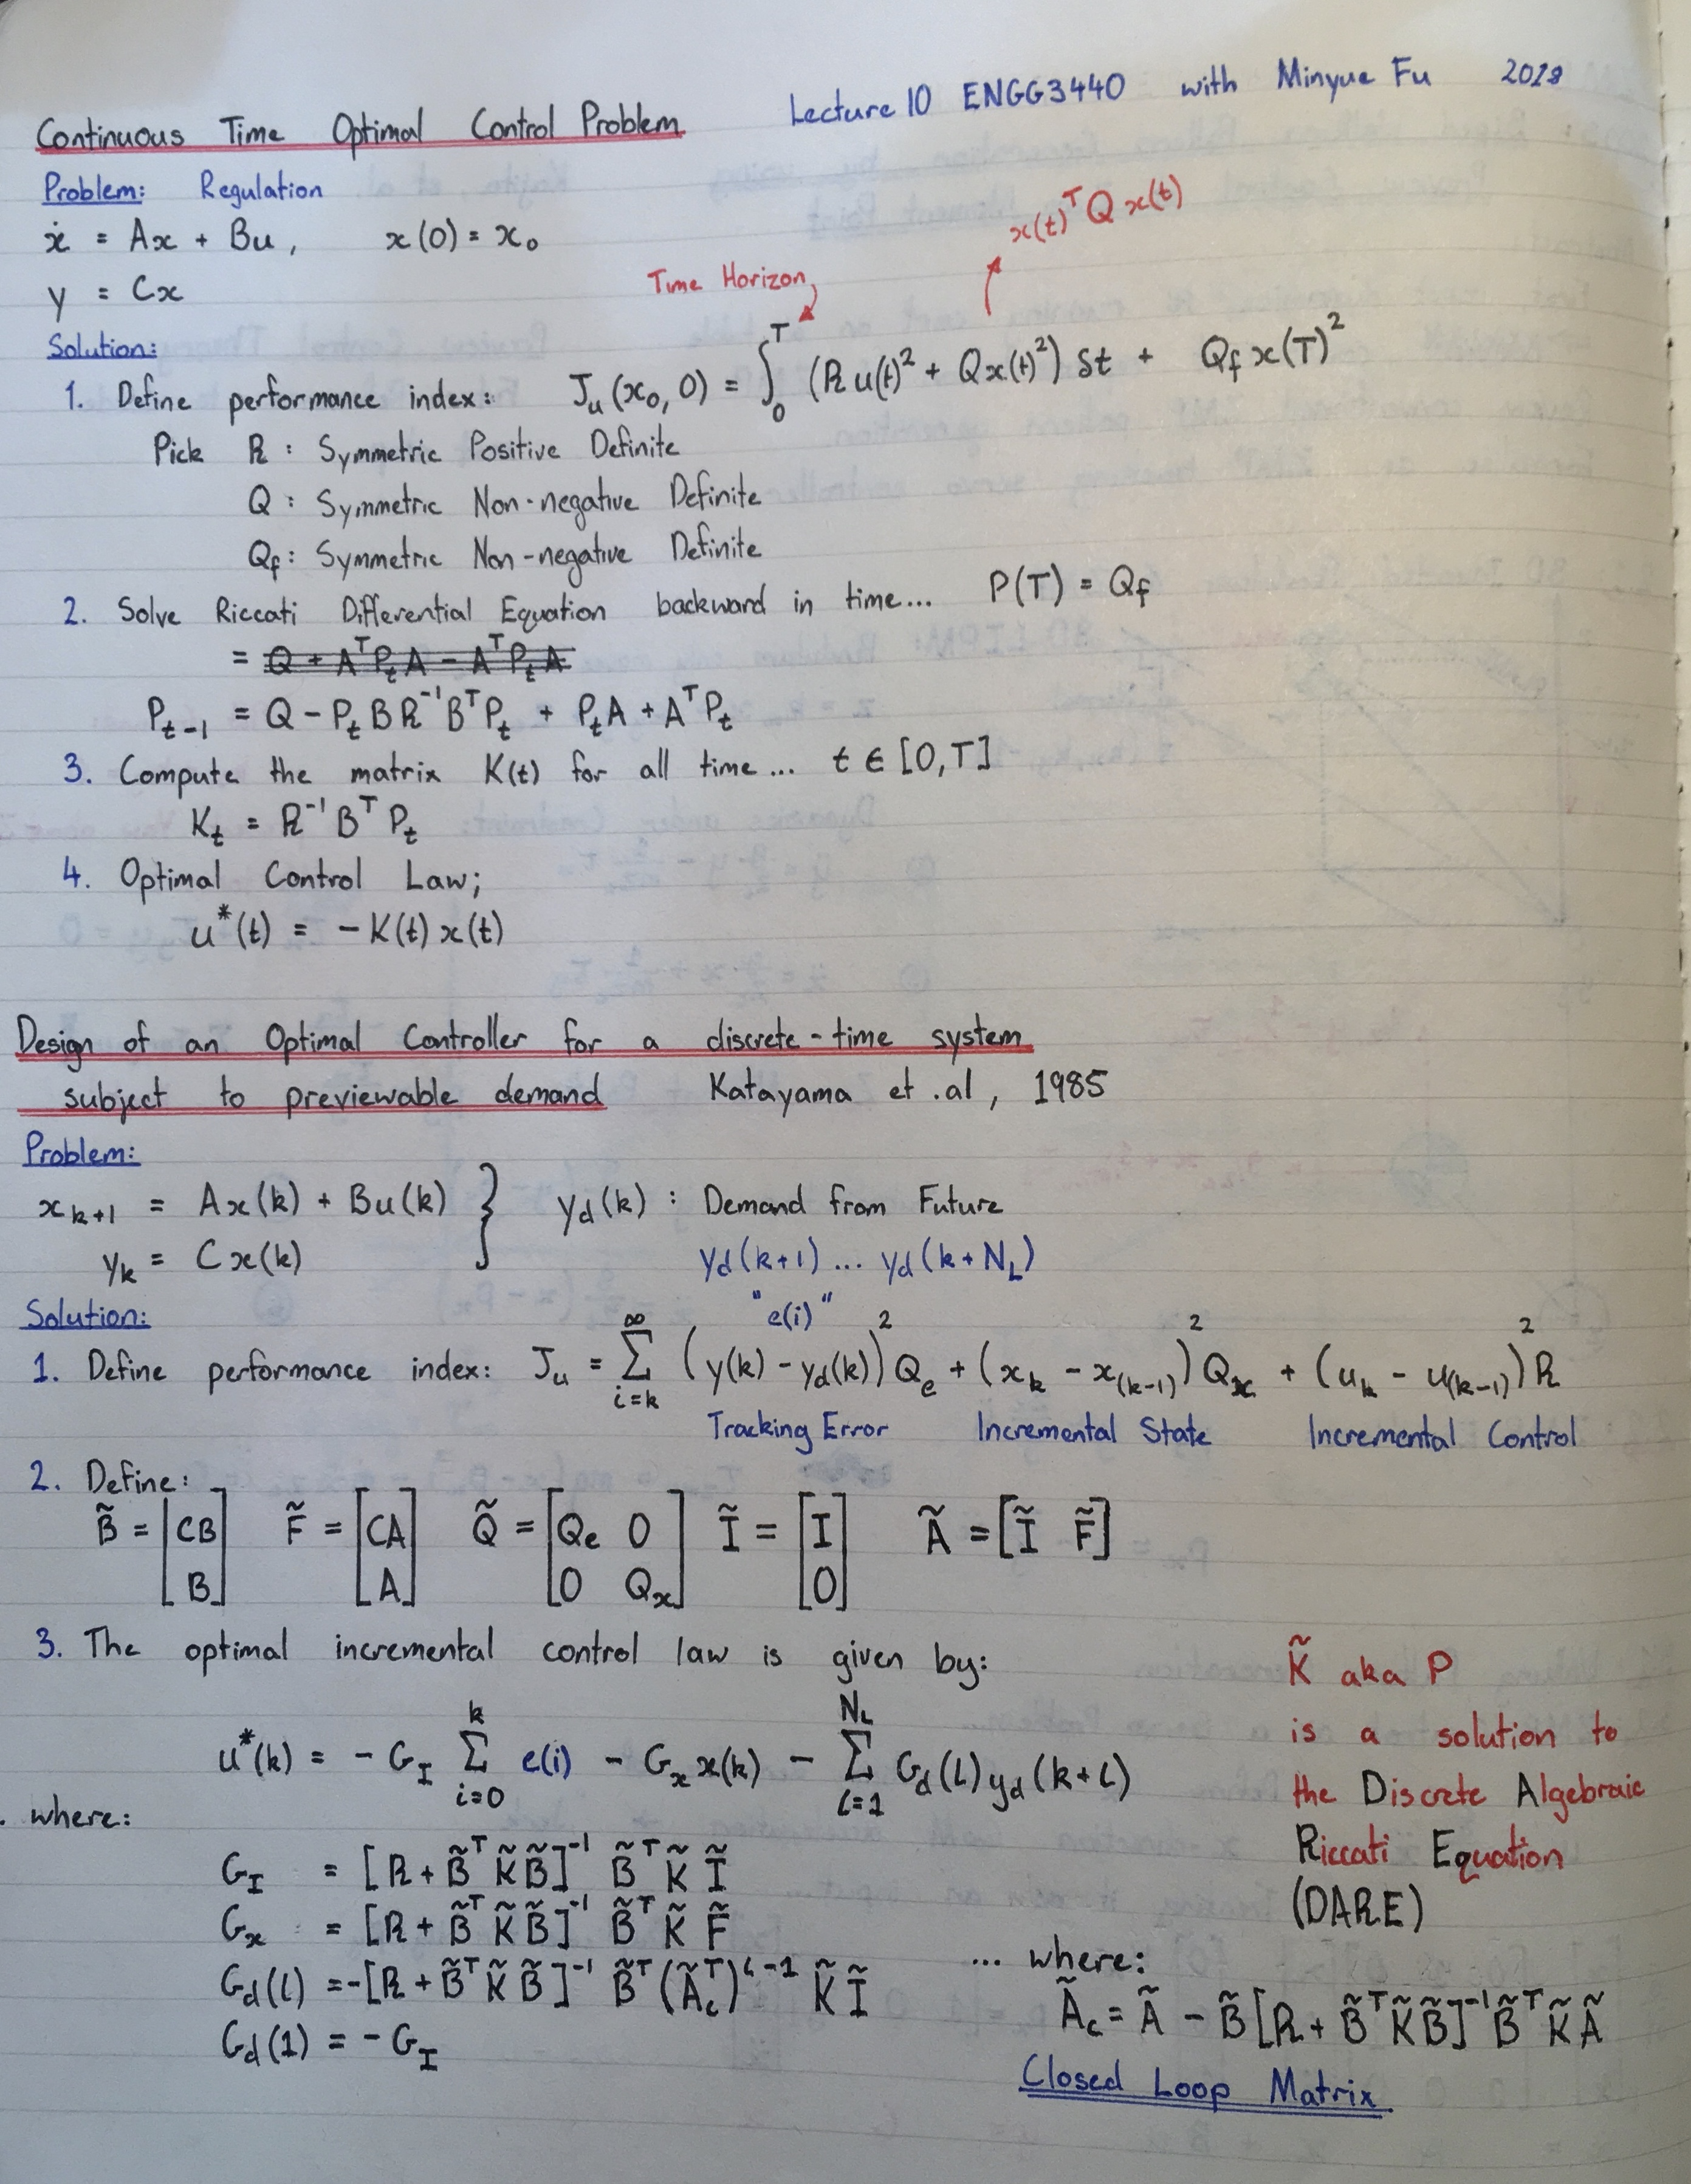
\includegraphics[width=.9\linewidth]{_figures/HAND_6_Preview.png}
		        \caption{Preview Control.}
		        \label{fig:APP_PREVIEW}
		    \end{center}
		\end{figure}
		\clearpage
		\newpage\section{Algorithms}\label{app:Algo}
		
\end{document}


%\lstinputlisting[
%    language=Matlab,
%    float=h,
%    numbers=left,
%    xleftmargin=1cm,
%    frame=shadowbox,
%    caption={Matlab serial communication example.\label{lst:matlabserial}},
%    morekeywords={try,catch}
%    ]{Code/serialtest.m}

%\begin{table}[h!]
%    \begin{center}\label{tab:MCHAProg}
%        \caption{Bachelor of Engineering Mechatronics First Year Program}\label{tab:notation}
%        {\footnotesize
%            \begin{tabular}{c l l l|}
%                \hline\hline \textbf{1st Year} & & \\
%                Semester & {Course Code} & {Course Name} \\ \hline 
%                1 & GENG1003 & Introduction to Procedural Programming \\
%                1 & GENG1500 & Introduction to Professional Engineering\\
%                1 & MATH1110 & Maths for Engineering, Science \& Technology 1
%\\
%                1 & PHYS1205 & Advanced Physics I\\ \hline
%                2 & CIVL1100 & Fundamentals of Engineering Mechanics\\
%                2 & ELEC1310 & Introduction to Electrical Engineering\\
%                2 & MATH1120 & Maths for Engineering, Science \& Technology 2 \\
%                2 & MECH1110 & Mechanical Drawing/CAD \& Workshop Practice\\ \hline
%            \end{tabular}
%        }
%    \end{center}
%\end{table}
